\section{Тело, брошенное под углом к горизонту}

%1
\AddProb Камень брошен с высоты $h$ под углом $\alpha$ к горизонту  со скоростью $v_0$. 
Какой угол $\beta$ будет составлять скоростью камня с горизонтом в момент падения на землю? Чему равна величина этой скорости? На каком расстоянии $s$ по горизонтали от основания точки запуска упадет камень? 

\AddProb С какой минимальной скоростью можно перебросить камень через здание высоты $H$ с куполообразной крышей радиуса $R$?

\AddProb Мальчик бросает камень в кота, сидящего на крае сарая. 
Через 1 секунду камень падает на землю в точку, находящуюся на одной вертикали с котом. 
На какой высоте находился кот?

\AddProb Мышонок стреляет из рогатки в кота, сидящего на ветке дерева. Через $t = 1$ с камень попадает в ветку прямо у лап кота. 
На каком расстоянии $s$ от мышонка находился кот, если известно, что векторы $v(0)$ и $v(t)$ взаимно перпендикулярны? 
Ускорение свободного падения $g$ = 10 м/с. Сопротивление воздуха пренебрежимо мало.

\AddProb (2005) Колесо радиуса $R$ катится по горизонтальной мокрой дороге со скоростью $v$. 
На какую максимальную высоту $h$ поднимаются капли воды, отрывающиеся от колеса? 
Какой должна быть минимальная скорость колеса, чтобы капелька, достигшая максимальной высоты, опустилась на то же самое место? 
Изменится ли высота $h$, если колесо будет катиться с пробуксовкой?

\begin{wrapfigure}{r}{5.0cm}
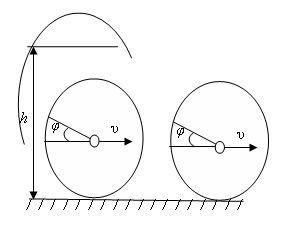
\includegraphics[width=5.0cm]{0205AngleWheel.jpg}
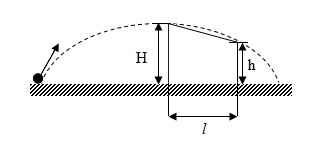
\includegraphics[width=5.0cm]{0209AngleHouse.jpg}
\end{wrapfigure}

%6
\AddProb Из двух точек, расположенных на одной высоте $h$ над землёй на расстоянии $l$ друг от друга, 
одновременно бросают два камня: вертикально вверх со скоростью $\vec{v}_1$ и горизонтально со скоростью $\vec{v}_2$. 
Каково минимальное расстояние между камнями в процессе их движения?

\AddProb Необходимо с поверхности земли попасть камнем в цель, расположенную на расстоянии $L$ по горизонтали на высоте $H$. 
С какой наименьшей скоростью это можно сделать? Трением пренебречь.

\AddProb (2004) При какой минимальной начальной скорости $v_0$ можно перебросить камень через дом с покатой крышей? 
Ближайшая стена имеет высоту $H$, задняя стена -- высоту $h$, ширина дома равна $l$.

\AddProb (2010) В сферической лунке прыгает шарик, упруго отражаясь от ее стенки в двух точках, расположенных на одной горизонтали. 
Промежуток времени при движении шарика слева направо равен $T_{1}$, а при движении справа налево -- $T_2$. Определите радиус лунки.

%11
\AddProb Из точек A и В, находящихся на одной горизонтальной прямой, одновременно бросили два камня с одинаковыми по модулю скоростями $v_0$ = 20 м/с. 
Один из камней полетел по навесной траектории, другой -- по настильной, но каждый попал в точку старта другого камня. 
Известно, что в точке А угол бросания $\alpha = 75^{\circ}$. 
Через какое время $\tau$ после старта расстояние между камнями станет минимальным? Чему равно это расстояние?

\AddProb (2008) В одной плоскости движутся две точки: точка 1 движется по прямой с постоянной скоростью $v_1$, 
а точка 2 -- с постоянной по модулю скоростью $v_2$, направленной все время на точку 1. 
Найти траекторию точки 2 и координату встречи точек 1 и 2. 
Считать, что в момент времени $t$ = 0 расстояние между точками $y_0$, а $\vec{v}_1$ и $\vec{v}_2$ перпендикулярны.
